% Visionner le code LaTeX

%% LyX 2.0.6 created this file.  For more info, see http://www.lyx.org/.
%% Do not edit unless you really know what you are doing.
\documentclass[english,french]{article}
\usepackage[T1]{fontenc}
\usepackage[latin9]{inputenc}
\usepackage{listings}
\usepackage{float}
\usepackage{graphicx}

\makeatletter

%%%%%%%%%%%%%%%%%%%%%%%%%%%%%% LyX specific LaTeX commands.
%% A simple dot to overcome graphicx limitations
\newcommand{\lyxdot}{.}

\floatstyle{ruled}
\newfloat{algorithm}{tbp}{loa}
\providecommand{\algorithmname}{Algorithme}
\floatname{algorithm}{\protect\algorithmname}

\makeatother

\usepackage{babel}
\makeatletter
\addto\extrasfrench{%
   \providecommand{\og}{\leavevmode\flqq~}%
   \providecommand{\fg}{\ifdim\lastskip>\z@\unskip\fi~\frqq}%
}

\makeatother
\addto\captionsenglish{\renewcommand{\algorithmname}{Algorithm}}
\addto\captionsfrench{\renewcommand{\algorithmname}{Algorithme}}

\begin{document}

\title{Rapport projet EDD - TSP}


\author{Delmas Rémi}


\date{16 avril 2014}

\maketitle
Adresse du dépôt git : https://github.com/azpown/TSP-Project

HowToCompile : cd build;cmake;(ctest)

\newpage{}


\part*{Introduction}

Le problème du voyageur de commerce (TSP) est un problème mathématique
qui consiste, étant donné un ensemble de villes séparées par des distances
données, à trouver le plus court chemin qui relie toutes les villes.
Ce problème est un problème NP-complet, il n'existe pour l'instant
aucun algorithme de résolution d'un tel problème en temps polynomial,
tous les algorithmes actuels ayant des temps exponentiel par rapport
a la taille des données d'entrée.

Aussi, la nécessité d'avoir des solutions approchées en temps polynomial
apparait immédiatement, l'obtention d'une solution exacte sur des
instances trop volumineuse n'étant pas envisageable.

Nous avons donc, au cour de ce projet, dévellopé deux heuristiques
, NearestNeighbour et MinimumSpanningTree, ainsi qu'un algorithme
de fournissant la solution exacte a une instance donnée.

Dans ce projet, nous avons utilisés des fichiers stockant les instances
de ce problème au format TSPLIB95, un autre aspect de ce projet a
également été de réaliser un parseur pour ce type de fichier, nous
restreignant néanmois a certaines instances ayant des attributs spécifiques.


\part*{Table des matières}


\section{Méthodes pour l'organisation}


\subsection{Le dépot de travail}

Afin de pouvoir travailler en simultané sur le même projet avec les
différents membres du groupe, nous avons choisit de mettre en place
un dépot git, sur la plateforme GitHub, dont l'architecture est disponible
en annexe.

Dans la forme, le fonctionnement de git est assez similaire a celui
de svn, mais pas dans la manière dont sont stockées les données. Nous
avons choisis git surtout car nous connaisions ces fonctionnalités,
et nous nous étions déjà servis pour de précédents projets.

Ce dépot est organisé en différents dossiers, les principaux étant
\texttt{src} et \texttt{include}.

Un dossier \texttt{build} est disponible sur le dépôt, pour que ne
pas encombrer la racine de ce dernier avec les différents fichiers
générés par le Makefile.


\subsubsection*{include}

Ce dossier contient uniquement les headers des différents fichiers
sources. Ce dossier est tag dans le CMakeLists comme étant le dossier
où trouver les headers lors de la compilation.


\subsubsection*{src}

Ce dossier contient les répertoires où sont les différents fichiers
sources, ainsi que les tests. Il contient également les différents
CMakeLists, permettant une génération des Makefile et l'automatisation
des tests.


\subsection{La construction logicielle}

Dans un premier temps, nous avons implémentés plusieurs Makefile afin
de généré nos éxécutables.

Cependant, leurs conception est assez hardu (afin d'avoir des makefiles
génériques), et l'exécution automatique des tests peu lisibles.

Nous avons ensuite, face a cette difficultée,choisit de mettre en
place un systeme de construction logicielle basée sur cmake, nous
permettant une compilation sans soucis, et l'utilisation de ctest,
très pratique pour lancer les tests unitaires.

Un CMakeLists.txt est présent dans le dépôt, indiquand les options
de compilation, le dossier source des header, et le dossier destination
des library.

Ce fichiers va lancé le CMakeLists de src, qui va créé les library,
les déplacés dans le dossier <fichierCourant>/lib et lancer les CMakeLists
des sous-dossiers de src, qui seront chargés de creer les tests, et
de fournir les EXPECTED\_VALUES qui détermineront le bon fonctionnement
ou non des différents tests.

\begin{figure}[H]
\setlength{\unitlength}{3mm} 
\begin{picture}(50,15) 
\put(0,5){$CMakeList.txt$}
\put(3,7){$depot$}
\put(10,5){\vector(1,0){5}}
\put(17,5){$CMakeList.txt$}
\put(20,7){$src$}
\put(27,5){\vector(1,0){5}}
\put(27,5){\vector(1,1){5}}
\put(27,5){\vector(1,-1){5}}
\put(33,5){$...$}
\put(33,10){$CMakeList.txt$}
\put(33,0){$CMakeList.txt$}
\put(33,12){$sous\ dossier \ src$}
\thinlines
\end{picture}\caption{Parcour cmake}


\end{figure}



\subsection{Génération de la documentation}

Pour la générisation automatique de la documentation nous avons décidé
d'utiliser Doxygen par l'intermédiaire de la commande doxywizard car
il est simple d'utilisation et fonctionne parfaitement. Nous avons
ainsi pu préciser dans le pdf obtenu après compilation du makefile
généré par doxywizard le nom, la version et le langage utilisé pour
le projet. La création automatique de la table des matières permet
d'accéder facilement aux informations dont on a la nécessité. Cette
documentation contient les informations indispensables pour qu'un
utilisateur extérieur au projet puisse utiliser ses diverses fonctionnalitées,
il contient notament les données membres des structures implémentées,
les descriptions des fonctions et les informations pour leur utilisation
(les paramètres qu'elles prennent, à quoi correspond l'objet qu'elles
renvoient, ....


\subsection{Méthodes de communication}

Durant la début de réalisation du projet, il nous est arrivé de ne
pas pouvoir communiquer les uns avec les autres, et que deux membres
du trînome travaillent sur le même algorithme, gachant ainsi du temps
qui aurait pût mieux être utilisé.

Nous avons donc mis en place un fichier texte TODO sur le dépot, régulièrement
mis à jour, contenant le travail que l'on a effectué, nos différentes
remarques sur l'avancement du projet et la travail de chacun avant
de pouvoir communiquer par des moyens plus standarts.

\begin{figure}[H]
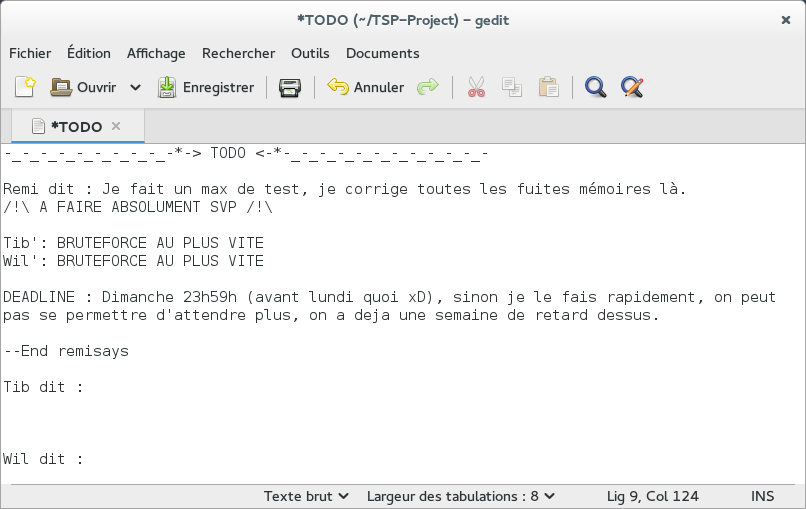
\includegraphics[scale=0.5]{capture-TODO}\caption{capture d'écran de TODO}
\end{figure}



\section{Présentation des structures usuelles.}

Il a fallut implémenté plusieurs structures de données afin d'effectuer
les différents traitement aboutissant aux divers algorithmes.

Les structures abordées dans ce paragraphe n'ont pas vraiment d'interêt
algorithmique, cependant, elle sont incontournables dans notre projet
car omniprésente. 


\subsection{Graphe}

Il s'agit d'une structure de basse, utilisée dans la plupart de nos
modules, contenant :

\begin{lstlisting}[basicstyle={\small},numbers=left,tabsize=3]
int taille_matrice_données;
double** matrice_données; 
\end{lstlisting}


Cette structure sert aux passages des données aux différents modules,
évitant ainsi de manipuler deux élements toujours associés.


\subsection{Arete}

Cette structure contient:

\begin{lstlisting}[basicstyle={\small},numbers=left,tabsize=3]
int ville_depart;
int ville_arrivée;
double distance_ville_depart_ville_arrivée
\end{lstlisting}


Elle nous permet d'évitée le passage de plusieurs paramètres, rendant
le code bien plus lisible.

Nos conteneurs ont été implémenté via délégation d'un module générique,
notre objectifs étant d'avoir le moins de duplication de code possible
entre les différentes heuristiques.

De plus, l'ajout d'une heuristique utilisant un conteneur déjà implémenté
sera bien plus aisée.


\section{Fonctionnement des algorithmes }


\subsection{Nearest Neighbour}

Le Principe de l'algorithme de NearestNeigbour est de parcourir un
graphe en passant par le voisin le plus proche du sommet actuel successivement
sans repasser par la même ville sauf pour la première et la dernière
qui sont identique pour faire un cycle puis de retourner la distance
totale obtenue.

\begin{figure}[H]


\centering{}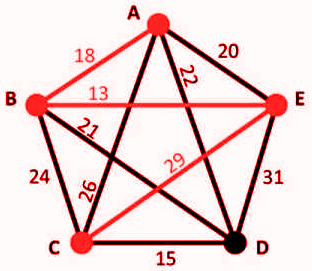
\includegraphics[scale=0.5]{NN}\caption{Illustration Nearest Neighbour en cour}
\end{figure}



\subsubsection*{Pseudo-code de l'algorithme:}

\begin{algorithm}[H]
\begin{lstlisting}[basicstyle={\small},numbers=left,tabsize=3]
NearestNeigbour:		
acc=0;
ville_precedement_NN=depart;
Tant que ville_valide_restante
	acc+=distance(ville_precedement_NN, pp_voisin(ville_precedement_NN));
	ville_precedement_NN=plus_proche_voisin(ville_precedement_NN);
fin Tant que;	  	 		
acc+=distance(dernierVisite,ville_precedement_NN);
return chemin_des_sommets_succesivement_visité;
\end{lstlisting}


\caption{Nearest Neighbour}
\end{algorithm}


Dans la pratique, cet algorithme renvoie souvent des résultats très
proches du chemin minimal (\textasciitilde{}+30\%) et est très rapide,
même sur des instances imposantes.


\subsection{Prim - MinimumSpanningTree}

L 'algorithme de Prim est un algorithme qui permet de trouver un arbre
couvrant minimal dans un graphe connexe (c'est à dire que tous ses
sommets sont liés) valué et non-orienté. 

Il part d'un sommet arbitraire puis fait grossir A 0 en y adjoignant
une arête de poids minimal qui le laisse connexe et sans cycle

Avec un parcour prefixe de cet arbre, on garentit $tailleChemin<2*tailleCheminMinimal$.

\begin{figure}[H]


\centering{}\includegraphics[scale=0.7]{220px-Minimum_spanning_tree\lyxdot svg}\caption{Arbre couvrant poid minimal}
\end{figure}


Cet algorithme forme un nouvel arbre sur l'ensemble des sommets du
graphe initial, tel que la somme des poids de ces arêtes soit minimale
càd, ayant une distance minimale.

Nous avons fait le choix d'implémenté cette algorithme, car sa compléxitée
théorique avec un tas min est très bonne : \foreignlanguage{english}{$O(nombreSommet{{}^2})$}


\subsubsection{Tas min}

Pour obtenir une telle complexitée, il faut utiliser un tas min comme
file de prioritée afin de déterminer quelle arete doit etre ajouter
au Minimum Spanning Tree.

La clé de chaque element stocké dans le tas est donc susceptible de
changer, et donc la position de ce dernier dans le tas également.

Nous n'avons dans un premier temps pas pris en compte ce paramètre,
ce qui nous a considérablement ralentit dans l'implémentation du module.

En plus de la structure du tas classique, il faut donc stocker avec
chaque élément l'indice du tableau du tas où sont stockés ces deux
derniers, on appelle un tel objet handle.

La structures des elements référencés dans le tas générique n'est
donc pas :

\begin{lstlisting}[basicstyle={\small},numbers=left,tabsize=3]
void* element_a_stock;
\end{lstlisting}
mais plutot :
\begin{lstlisting}[basicstyle={\small},numbers=left,tabsize=3]
void* element_a_stock;
int handle_sur_tableau; /* compris entre 0 et taille_tas */
\end{lstlisting}



\subsubsection{Arbre ``Planaire''}

L'implémentation de l'arbre nous permet de stock le Minimum Spanning
Tree. Nous appelons un arbre ``planaire'' un arbre stockant des
noeuds de la forme:

\begin{lstlisting}[basicstyle={\small},numbers=left,tabsize=3]
type Noeud:
	void* element_a_stock;
	Noeud* Noeud_pere;
	Noeud* Noeud_premier_fils;
	Noeud* Noeud_frere;
\end{lstlisting}


où un pere accede a ces fils via acces a son fils puis aux freres
de ce dernier jusqu'a obtenir le fils choisis.

Notre arbre délégué devant contenir des entiers, nous avons dût mettre
en place un mécanisme afin de pouvoir stocker des types non pointeur.

Nous allouons donc la mémoire de l'int a stock, puis nous stockons
sa référence dans le tableau. Le mécanisme inverse doit etre effectué
afin de pouvoir lire l'entier a la sortie et libérer la mémoire allouer.


\subsubsection{Pseudo-code de l'algorithme}

\begin{algorithm}[H]
\begin{lstlisting}[basicstyle={\small},language=C,numbers=left,tabsize=3]
Prim-MST:

a = choisir_arete_min_depuis(depart,tab_arete_disponible);
ajouter(a,tas_min,0) // (arete,tas,clée);
Pour chaque s tel que s != a 
	ajouter(a,tas_min,distance(a,s));
Tant que !est_vide_tas(tas_min)
	s=extraire_min(tas);
	ajout_arbre(Arbre_int,get_depart(s),get_arive(s)) // (arbre,pere,elem)
	Pour tout voisin v de s: //(càd tout le monde,d'ou la compléxité)
		Si v !appartient_tas(tas) && distance(s,v) < cle(tas_min,v): // Handle nécces.
			set_depart_arete(v,get_arrive(s)); // Modification de l'arete
			diminuer_cle_tas(tas_min,v,distance(s,v));
		fin Si;
	fin Pour;
fin Tant que;
return parcour_prefixe(Arbre);
\end{lstlisting}


\caption{Prim - MST}
\end{algorithm}


L'algorithme est relativement rapide, cependant, son implémentation
n'est pas chose aisée, car elle passe par l'implémentation de deux
conteneurs.

Il est prouvé qu'il s'agit d'une 2-approximation, cependant, ces résultats
sont bien souvent moins bon que Nearest Neighbour.


\subsection{Brute Force Branch\&Bound}

L'algorithme Branch and Bound est une amélioration du Brute Force
naïf classique, connu dans beaucoup de domaine de l'informatique (ex
: réseau). Plutôt que parcourir et tester tous les parcours possibles
comme sa version simplifiée, il calcule à tout instant la distance
du parcours qu'il teste et avorte le test si la distance parcourue
au moment l'on dépasse la distance la plus courte enregistrée pour
un parcours complet. Cet algorithme épargne ainsi des tests à l'utilisateur
et diminue grandement le temps d'exécution par rapport à un brute
Brute Force naïf. Sa complexitée n'est en revanche pas polynomiale,
des tests sur de grande instance (+1000) deviennent extrèmement compliqués,
meme sur des machines puissantes et en parallélisant les parcours
(une utilisation du GPU serait particulièrement intérésante).

Le pseudo-code de cet algorithme récursif étant assez générique, nous
ne l'expliciterons pas ici.

notre algorithme effectue un parcours d'un tableau de booléen ou l'indice
du boolean indique si la ville est déja dans le chemin ou pas, en
mettant indisponibles les villes sur lesquelles il est déjà passé,
tout en vérifiant à chaque instant que la meilleure distance enregistrée
et inférieure a celle du chemin en cour.

A la fin du travail de l'appel, on remet le tableau dans son état
avant son appel afin de restaurer le contexte de l'appellant (et ainsi
avec un complexitée en espace minimale).


\section{Parsing}

Nous avons travaillé dans ce projet avec des fichers d'instance de
type TSP, d'où la nécessité de la création d'un fichier servant à
l'implémentation d'un parser qui va récuperer les différents champs
du-dit fichier. Les différents champs doivent etre présent afin de
valider le parsing, sinon un message d'erreur s'affiche sur la sortie
d'erreur standarts, et la mémoire est libérer. Il faut se servir des
accesseurs (les get) pour acceder à ces données par la suite.

Notre parseur se basse sur les fonctions getline (C++) et sscanf (allocation
dynamique de mémoire via \%ms) afin de récupérer efficacement le contenue
du fichier cible.

\begin{figure}[H]


\includegraphics[scale=0.5]{extsp}\caption{Exemple fichier .tsp}


\end{figure}

\end{document}
